\newpage

\section*{ $^{56}$Fe(n,p)$^{56}$Mn }

Power Level: 100 kW(th) \\
Time at Power: 60.0 s \\
Wait Time:  2.0 h \\
Counting Time: 60.0 m \\
Total Activity at Removal: 5.63e-03 $\mu Ci$

\begin{table*}[h]
\centering
\begin{tabular}{ |c|c|c|c|c|c| }
 \hline
 Position & Mass $mg$ & Counting Activity $\mu Ci$ & Area (Counts) & Error \% \\
 \hline 
 1 & 1.18 & 7.58e-04 & 1.89e+02 & 7.2772 \\ 
\hline
 2 & 1.18 & 8.93e-04 & 2.22e+02 & 6.7046 \\ 
\hline
 3 & 1.18 & 5.66e-04 & 1.41e+02 & 8.4192 \\ 
\hline
 4 & 1.18 & 1.96e-04 & 4.88e+01 & 14.3197 \\ 
\hline
\end{tabular}
\end{table*}

\begin{figure}[h]
\centering
\begin{subfigure}{.5\textwidth}
  \centering
     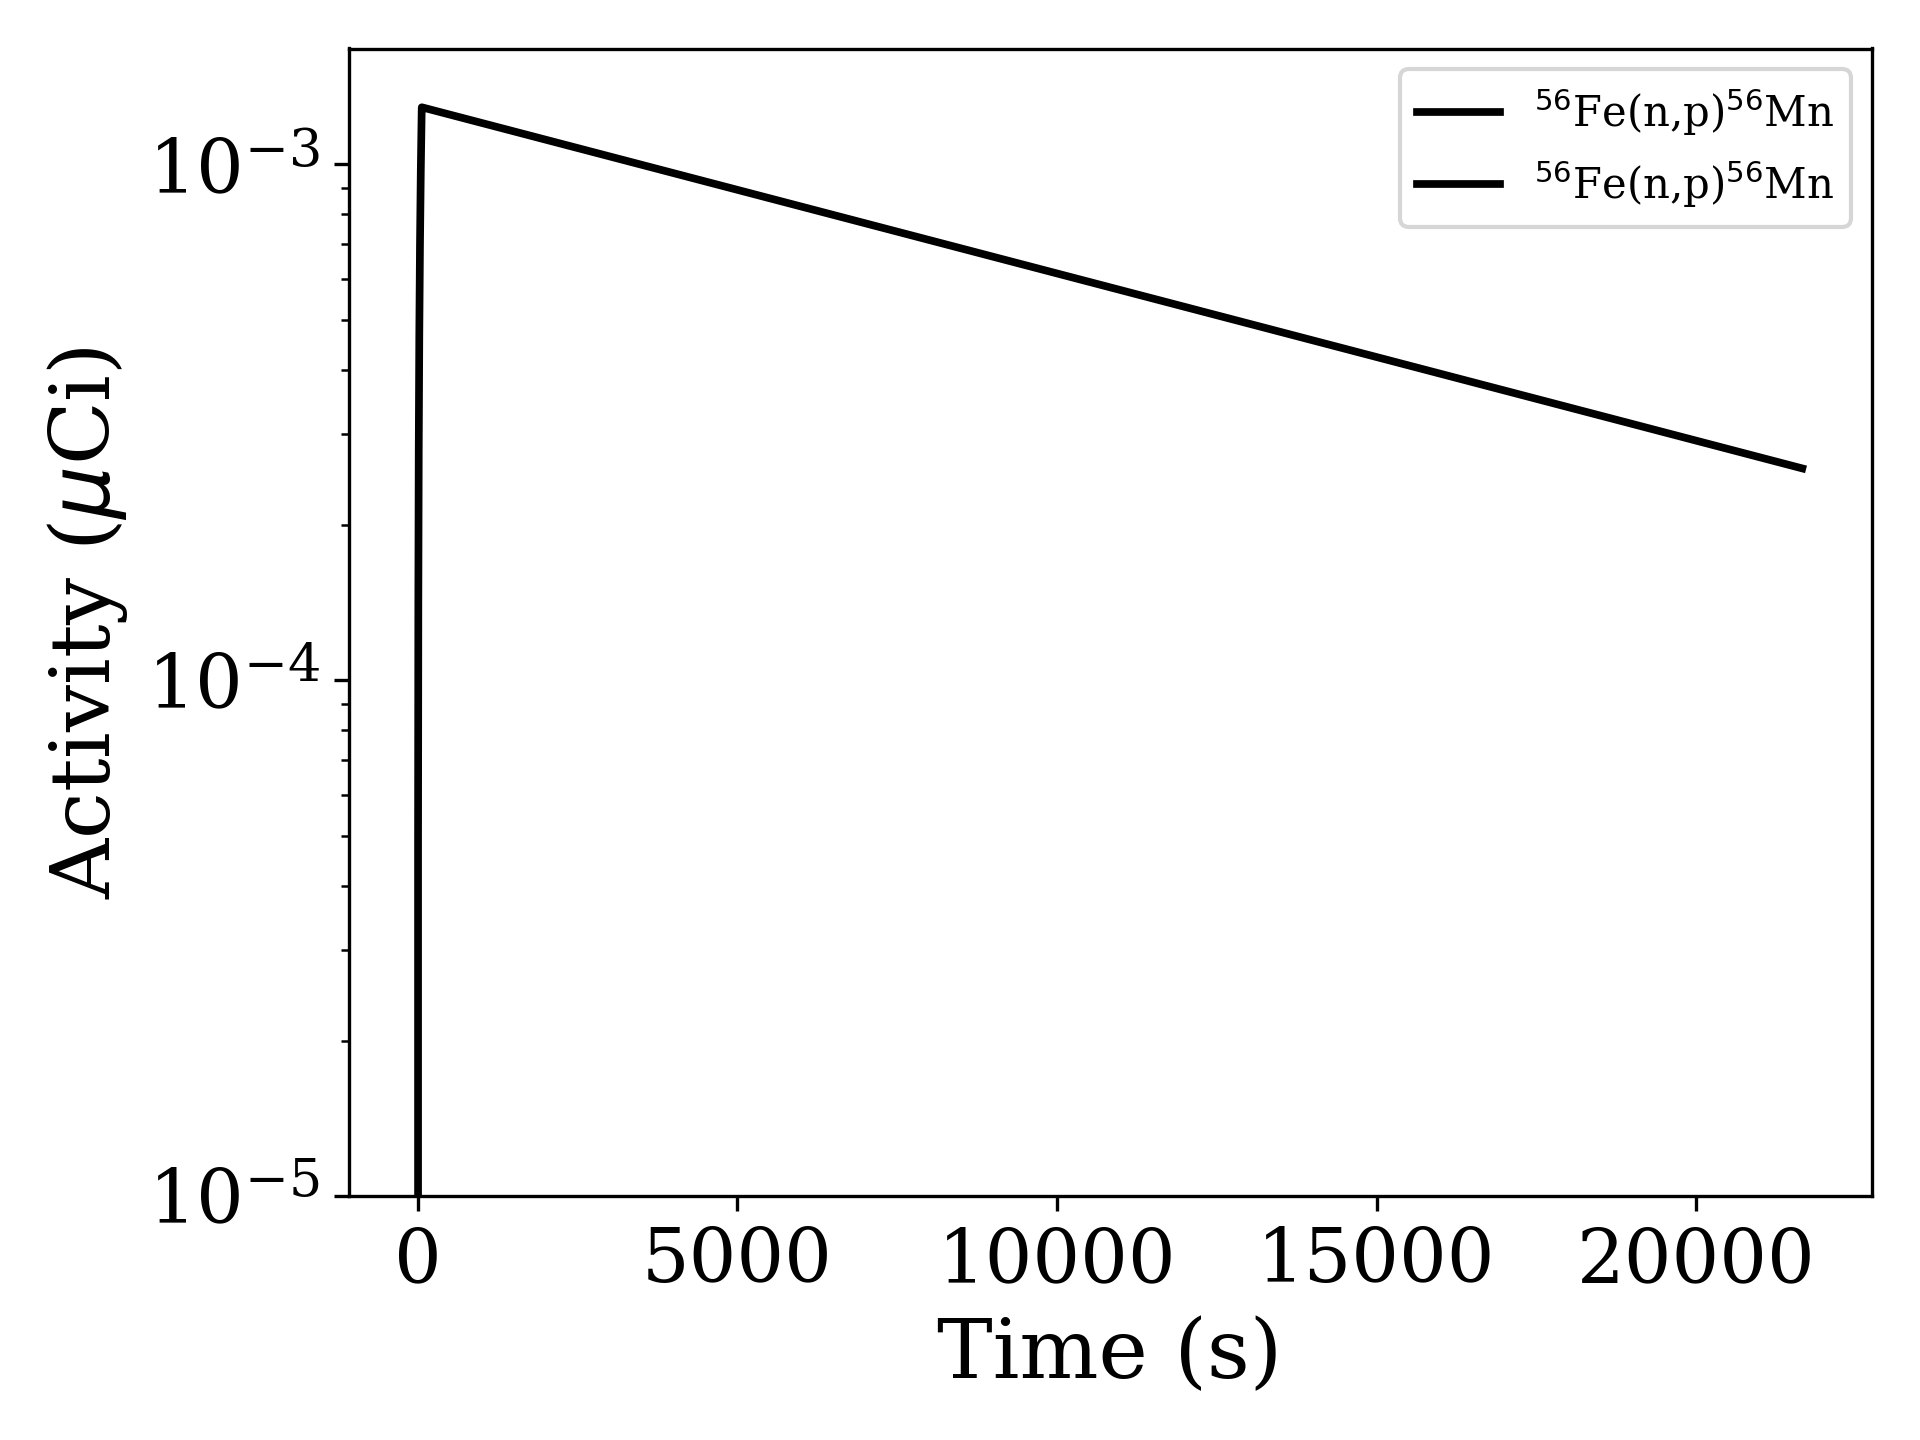
\includegraphics[width=.8\textwidth]{plot/Fe-56(n,p)Mn-56_library1} 

  \caption{A subfigure}
  \label{fig:sub1}
\end{subfigure}%
\begin{subfigure}{.5\textwidth}
  \centering
     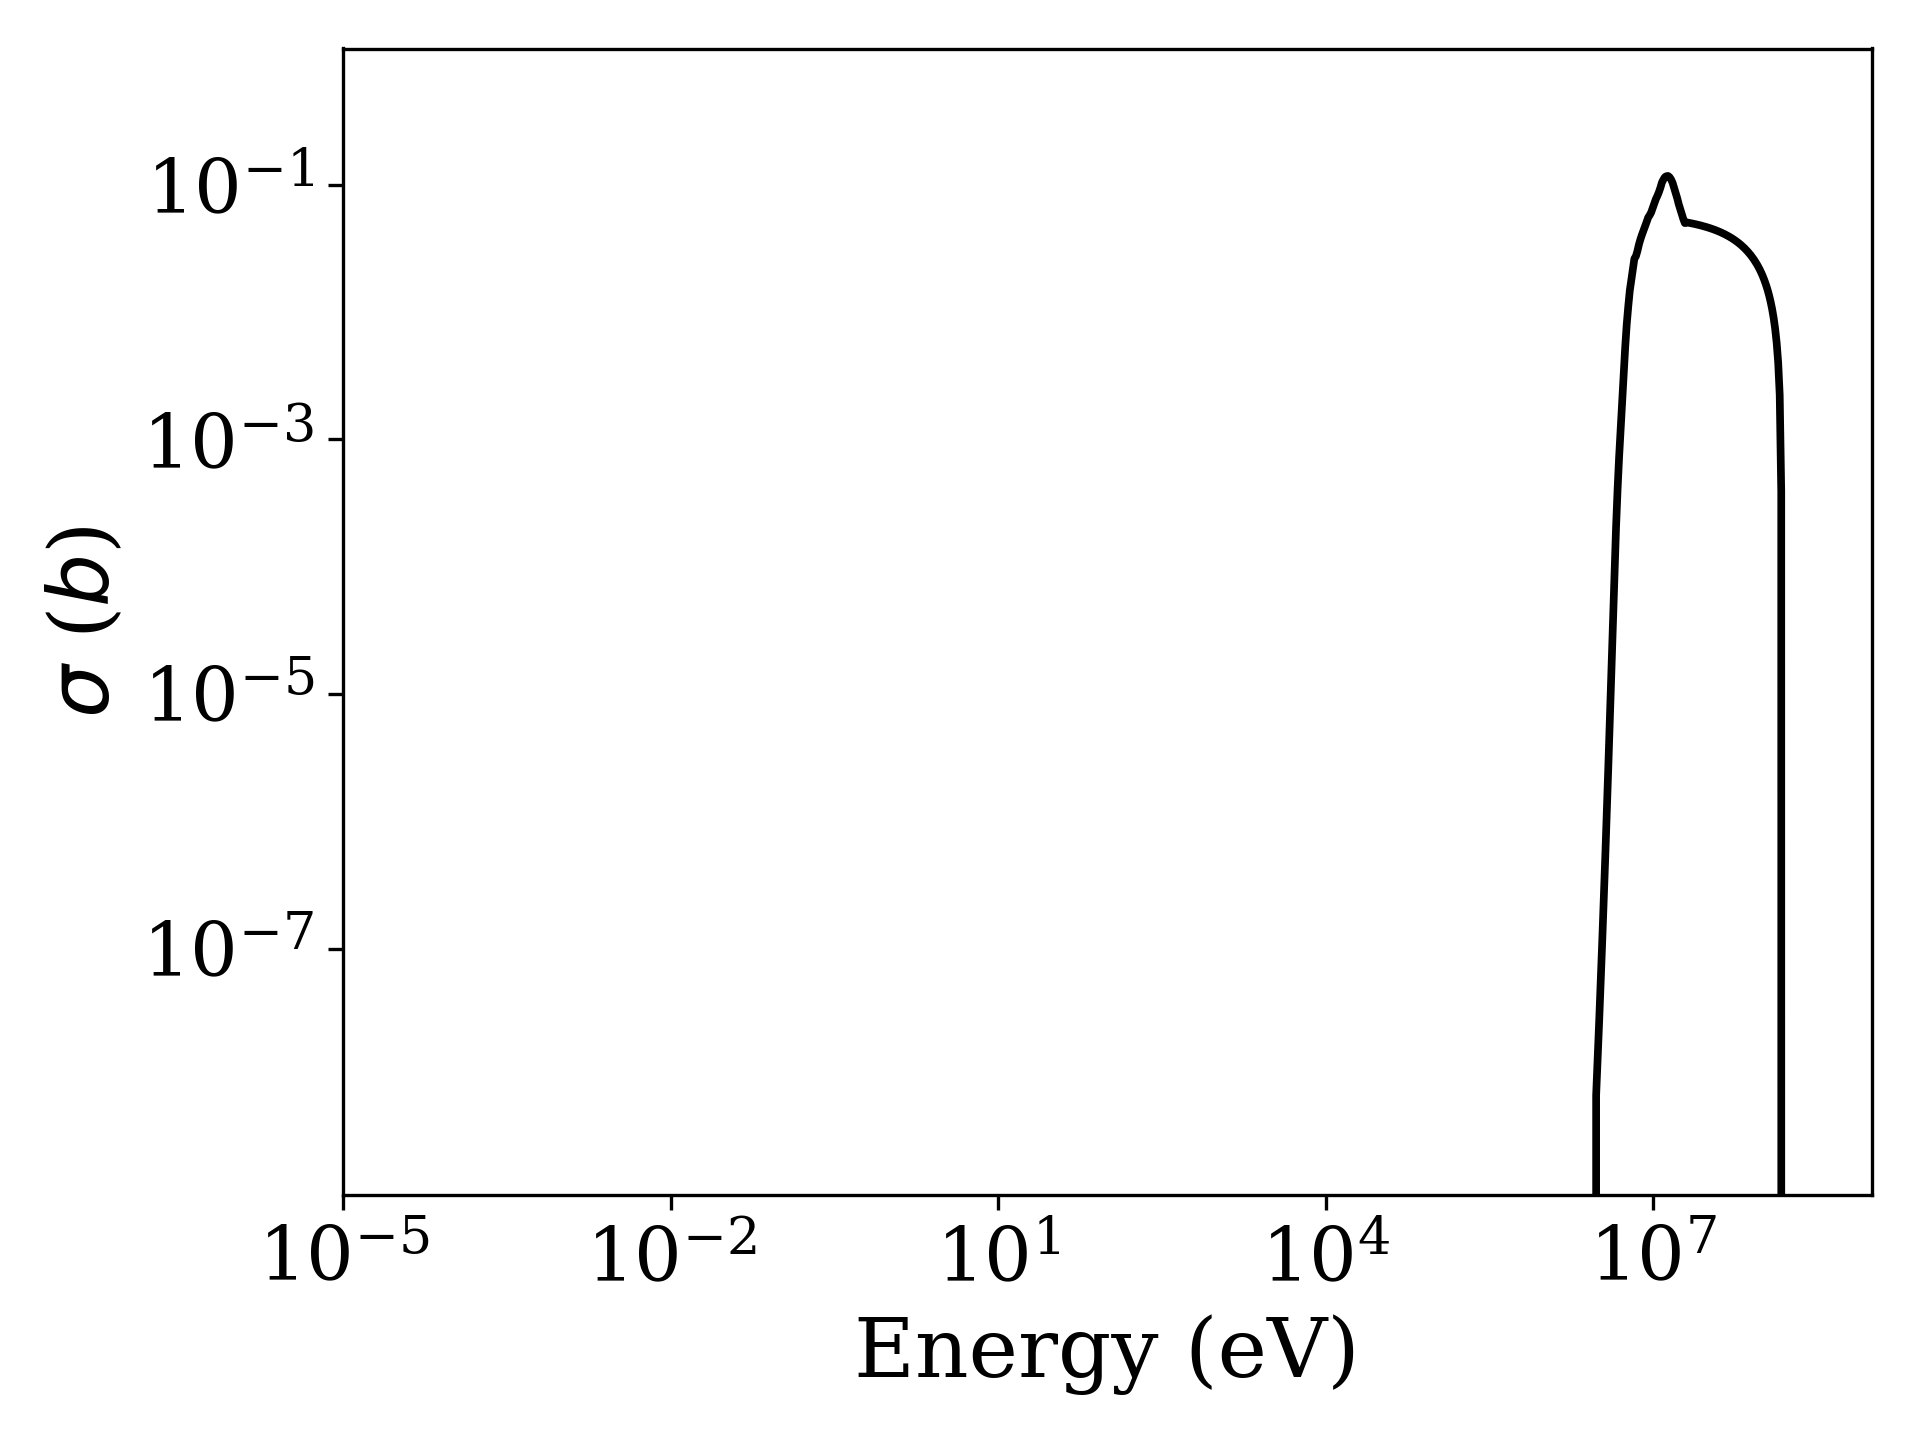
\includegraphics[width=.8\textwidth]{plot/Fe-56(n,p)Mn-56} 

  \caption{A subfigure}
  \label{fig:sub2}
\end{subfigure}
\caption{A figure with two subfigures}
\label{fig:test}
\end{figure}

\begin{table*}[h]
\centering
\begin{tabular}{ |c|c|c|c|c|c|c| }
 \hline
 Reaction & T$_{1/2}$ & ROI (eV) & Important Gammas (keV) \\
 \hline 
 $^{56}$Fe(n,p)$^{56}$Mn &  2.6 h & 5.58e+06, 1.16e+07 & 1810.726(0.269) \\ 
\hline
\end{tabular}
\end{table*}
